\documentclass[a4paper, 14pt]{extarticle}
\usepackage[top=1in, bottom=1in, left=1in, right=1in]{geometry}
\usepackage{amsmath}
\usepackage{amssymb}
\usepackage{graphicx}
\usepackage{fontspec}
\usepackage{hyperref}
\usepackage{tikz}
\usepackage{fontspec}
\usetikzlibrary{calc,decorations,patterns,arrows,decorations.pathmorphing,positioning}
\definecolor{pltblue}{HTML}{1F77B4}
\tikzset{every picture/.style={/utils/exec={\fontspec{Pretty Neat}}}}
\setmainfont{Pretty Neat}

\makeatletter
\pgfset{
  /pgf/decoration/randomness/.initial=2,
  /pgf/decoration/wavelength/.initial=100
}
\pgfdeclaredecoration{sketch}{init}{
  \state{init}[width=0pt,next state=draw,persistent precomputation={
    \pgfmathsetmacro\pgf@lib@dec@sketch@t0
  }]{}
  \state{draw}[width=\pgfdecorationsegmentlength,
  auto corner on length=\pgfdecorationsegmentlength,
  persistent precomputation={
    \pgfmathsetmacro\pgf@lib@dec@sketch@t{mod(\pgf@lib@dec@sketch@t+pow(\pgfkeysvalueof{/pgf/decoration/randomness},rand),\pgfkeysvalueof{/pgf/decoration/wavelength})}
  }]{
    \pgfmathparse{sin(2*\pgf@lib@dec@sketch@t*pi/\pgfkeysvalueof{/pgf/decoration/wavelength} r)}
    \pgfpathlineto{\pgfqpoint{\pgfdecorationsegmentlength}{\pgfmathresult\pgfdecorationsegmentamplitude}}
  }
  \state{final}{}
}
\tikzset{xkcd/.style={decorate,decoration={sketch,segment length=0.5pt,amplitude=0.5pt}}}
\makeatother

\usepackage{etoolbox}
\AtBeginEnvironment{tabular}{\fontspec{Pretty Neat}}

\setlength{\parindent}{0pt}
\setlength{\parskip}{0.5em}

\begin{document}

\section*{\fontspec{Pretty Neat}Efficient Representation of Social Networks}

You're studying social networks and need to find an efficient way to store and process connection data. Let's explore different representations using this small social network:

\begin{center}
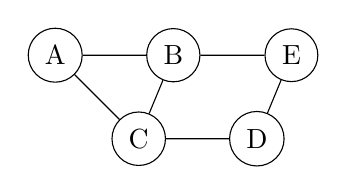
\begin{tikzpicture}[node distance=1.5cm]
    \node[draw, circle] (A) {A};
    \node[draw, circle] (B) [right of=A] {B};
    \node[draw, circle] (C) [below right of=A] {C};
    \node[draw, circle] (D) [right of=C] {D};
    \node[draw, circle] (E) [right of=B] {E};
    \draw (A) -- (B) -- (C) -- (D) -- (E) -- (B);
    \draw (A) -- (C);
\end{tikzpicture}
\end{center}

{\bf Question 1}:
Create a 5x5 grid where both rows and columns represent individuals (A to E). Mark friendships with a 1, and non-friendships with a 0. What are the advantages and disadvantages of this representation?

\vspace{10em}

{\bf Question 2}:
For each person, create a list of their friends' IDs. For example, A's list would be [B, C]. How does this representation compare to the grid in terms of efficiency?

\vspace{8em}

{\bf Question 3}:
We can optimize this representation further. Create three lists:
\begin{enumerate}
    \item A combined list, called \texttt{pointers}, of all friends
    \item A list, called \texttt{indices}, that shows where each person's friend list starts in the combined friend list. For example, if A has 2 friends and B has 3 friends and we combine the lists in order of A, B, C, D, E, B's list would start at index 2 in the combined list, and C's list would start at index 5.
    \item A list, called \texttt{data}, of 1's with the same length as the combined friend list
\end{enumerate}
Hint: Start the first list with 0, and for each subsequent entry, add the number of friends the previous person has.

\vspace{10em}

{\bf Question 4}:
Using the representation you created in Question 3, how many friends does C have using the \texttt{pointres} list?

\vspace{3em}

{\bf Question 5}:
List D's friends using the \texttt{pointers} and \texttt{indices} lists.

\vspace{3em}

{\bf Question 6}:
How many total friendships are in the network using the \texttt{data} list?

\vspace{3em}

{\bf Question 7}:
A makes a new friend with E. How would you modify your representation to reflect this change?

\vspace{8em}


\end{document}